\chapter{Team 7 Agent Design}\label{team_7_agent_design}

\section{Overview}
\label{sec: Team 7 Overview}
This chapter outlines the design and findings of Team 7's agent. The primary goal of team 7 was to emulate human behaviour closely and to replicate the normal variation in personality types exhibited in a typical human population. This would then enable analysis into whether particular personality types exhibited particular behavioural patterns or are more conducive to self organisation and thus acheiving the goal of sustainability in a collective action problem.

\section{Agent Design}
\label{sec: Agent Design}
There are 3 key elements that define the agent: its personality, behaviour and memory. The personality defines a given agent at its core, and for the purpose of this experiment is kept constant throughout a given simulation. An agents behaviour is influenced by its personality, memory (a record of its experiences) and the environment. The environment can include current floor, food available and interaction with other agents. The personality and behaviour then combine to influence the various decisions that the agent makes over the course of the simulation. 
This basic agent framework is illustrated in \Cref{agent_flow}.

\begin{figure}[H]
    \begin{center}
        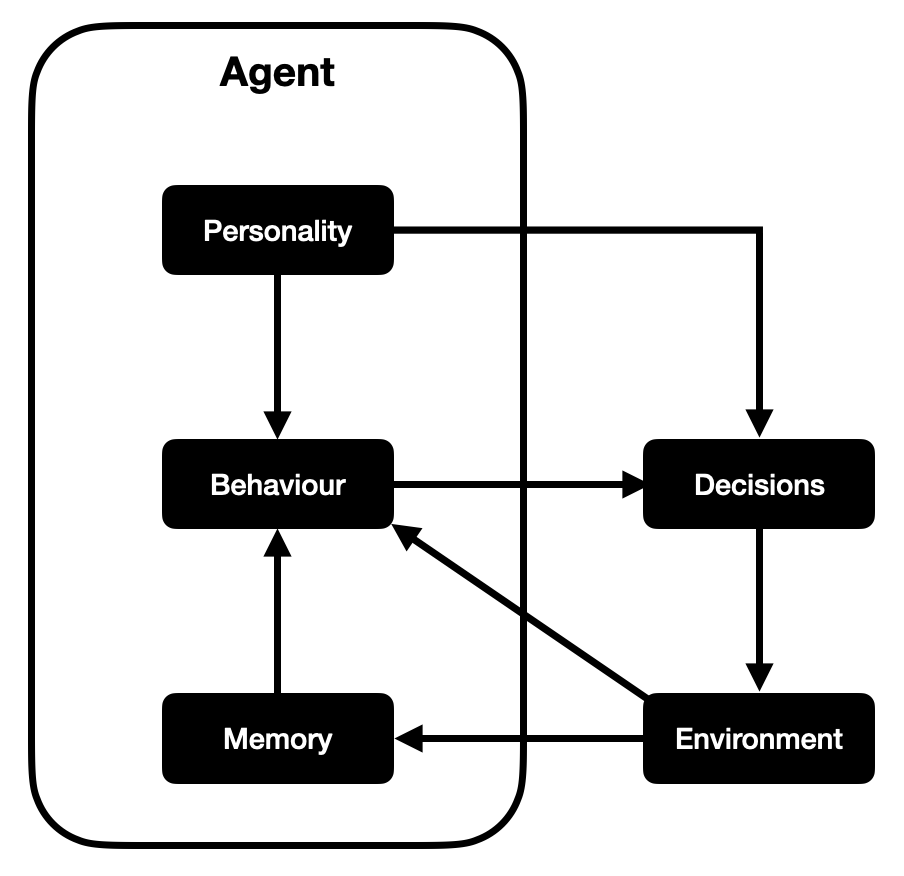
\includegraphics[width=6cm]
        {009_team_7_agent_design/Images/agent_flow.png}
    \end{center}
    \caption{Agent framework.}
    \label{agent_flow}
\end{figure}

\subsection{Personality Traits}
\label{subsec: Agent Design}
The use of personality traits to attribute human characteristics to our agents is a construct derived from Robert R. McCrae and Paul Costa's 5 factor theory of personality. McCrae and colleagues discovered that the big five traits are surprisingly universal which was confirmed by a study that looked at people from more than 50 different cultures. They determined that the five personality traits could be used to accurately model the human psychological framework.

The five personality dimensions consist of: 
\begin{itemize}
    \item  \textbf{Openness}: The degree to which an individual is willing and eager to have new experiences. This also has implications for creativity and problem solving. An individual with low openness will behave more conservatively and will be less welcoming to change. 
    
    \item  \textbf{Conscientiousness}: The degree of conscientiousness of an individual determines their level of organization, discipline and thoughtfulness. Conscientious individuals are also more strategic and forward thinking. 
    
    \item  \textbf{Extraversion}: Extraversion is the extent to which an individual is willing and eager to socialise and interact with other individuals. An extroverted individual is more likely to occupy positions of leadership and influence. 
    
    \item  \textbf{Agreeableness}: An individual with high agreeableness will exhibit greater degrees of kindness, trust, and altruism. On the other hand, an individual with low agreeableness will demonstrate a lack of sympathy and might be spiteful or manipulative towards others. 
    
    \item  \textbf{Neuroticism}: The neuroticism trait dictates the emotional stability of an individual. A greater value of this is associated with greater proneness to anxiety, irritability and mood swings. In the extreme case, individuals can experience regular fluctuations in their character. Therefore, an agent that is high in Neuroticism will commit actions that may seem unreasonable or illogical. 
\end{itemize}

Any time a new agent is deployed it is initialised with a value for these traits ranging from 20-80. We did this in order to exclude extreme personality traits on either end. The personality traits assigned to an agent are innate and unchanged for the duration of the simulation. This is done in order to emulate how traits remains fairly constant over a person's life.

\subsection{Behavioural Traits}
\label{subsec: Behaviour}
In contrast to personality traits, behavioural characteristics of an agent change over the course of the simulation. The behaviours are initialized based on the agent's personality traits and can range from 0-100 over the lifetime of the agent. These behaviours are then updated daily by environmental factors such as food availability, floor changes and interactions with other agents. 

The behaviour characteristics are described below:
\begin{itemize}
    \item  \textbf{Greediness}: This is the degree to which an agent behaves selfishly, specifically with regards to the amount of food it takes. The greediness value is initialised by the agent's agreeableness score meaning that high agreeableness will result in low initial greediness and vice versa. The greediness value is subsequently adjusted throughout the simulation run by the following factors: 
    
    \begin{itemize}
        \item Being in a critical health state increases greediness.
        \item Eating no food increases greediness by a quadratic factor with respect to the number of days since the last food intake.
        \item Agents display increased levels of greediness in response to being placed at a lower floor during the reshuffle and vice versa. The degree to which this changes is dependent on the openness of said agent.  
        \item Based on past experience, if the agent expects food shortages on a new floor, there will be an additional boost to greediness. This adjustment has a greater impact if the agent has high level of conscientiousness.
        \item Neuroticism can cause sporadic daily fluctuations in the greediness of an agent. A higher neuroticism results in more substantial daily changes of the relevant behaviours.
    \end{itemize}
    
    \item  \textbf{Kindness}: An agent with a high kindness value will demonstrate greater sympathy for other agents and will be more supportive of the wider social cause. Kinder agents will take less food and will be more likely to collaborate with other agents. 
    
    Similar to greediness, kindness is initialised by the agent's agreeableness score meaning that high agreeableness will result in high initial kindness. The kindness value is subsequently adjusted throughout the simulation run by the following factors:
    
    \begin{itemize}
        \item Agents display increased levels of kindness in response to being placed at a higher floor during the reshuffle and vice versa. The degree to which this changes is dependent on the openness of said agent. A lower the openness the greater the change.
        \item Neuroticism can also result in sporadic daily fluctuations in the kindness of an agent. A higher neuroticism results in more substantial daily changes of the relevant behaviours. 
    \end{itemize}
    
    \item  \textbf{Responsiveness}: 
    This behaviour influences the likelihood of an agent accepting the treaties of other agents. It is initialized as the average of openness, extraversion, and agreeableness. 
    
    In the current implementation, the responsiveness trait does not vary during the simulation. In an implementation where dishonesty is factored in, the agent would keep record of the trustworthiness of each agent that it interacts with. If other agents are largely untrustworthy, overall responsiveness would go down proportionally. 
    
\end{itemize}

The effect of personality traits on the behaviourial charactersitcs are described below:
\begin{itemize}
    \item  \textbf{Openness}: A high openness score means that agents are less impacted by floor changes and thus its behavioural characteristics are not varied as much. Conversely, a low openness score means an agent is significantly impacted by change such as arriving at a lower floor which increases their greediness more than it would an agent with a higher openness score. Openness also influences responsiveness, which dictates how much an agent is willing to accept or requests or treaties.
    
    \item  \textbf{Conscientiousness}: A high conscientiousness score means an agent will demonstrate greater learning from its experiences, as it will identify underlying trends in these experiences in order to make better decisions. A more planning-oriented agent of such will also give greater importance to collaborating with other agents.
    
    \item  \textbf{Extraversion}: Extraversion affects the responsiveness and a high score increases the likelihood of positive social interaction such as accepting requests or treaties. 
    
    \item  \textbf{Agreeableness}: Greediness and kindness are initialised by agreeableness and scaled accordingly. Agreeableness also has influence over responsiveness in the same way that openness and extraversion do.
    
    \item  \textbf{Neuroticism}: Neuroticism creates random day-to-day volatality in the greediness and kindness of an agent. Since greediness and kindness directly control the amount of food taken, an agent with higher neuroticism may intend to take an inadequate or excess amount of food.
\end{itemize}


\subsection{Operational Memory}
\label{subsec: Operational Memory}
The memory structure of the agent behaves analogously to human memory. It serves to store experiences and data acquired across the lifespan of the agent. These experiences and data serve to influence the agent's behaviour, inform it's decisions, and enhance its survival and organisation capabilities. 
Below is a description of all the elements of information stored in the agent's memory:

\begin{itemize}
    \item  \texttt{orderPrevFloors}: A chronologically ordered list of the floors that the agent has been in. 
    \item  \texttt{prevFloors}: A map of all the floors that the agent has experienced. This keeps track of the number of days spent on each given floor and the average food that was available whilst the agent was on that floor.
    \item  \texttt{currentDayonFloor}:The number of days the agent has spent on the current floor.
    \item  \texttt{currentFloorRisk}: This is the level of risk to the survival of the agent associated with the current floor. 
    \item  \texttt{daysHungry}: The number of consecutive days the agent has not consumed food.
    \item  \texttt{seenPlatform}: This variable is used to remember if the agent has seen the platform. The agent uses this to decide when to prepare for a new day.
    \item  \texttt{prevAge}: The age of the agent on the previous day.
    \item  \texttt{prevHP}: A record of the HP at the end of the previous day.
    \item  \texttt{foodEaten}: The amount of food consumed the previous day.
    \item  \texttt{receivedReq}: This is a variable that indicates whether the agent has decided to abide by a request made in a message. A false value indicates that no requests have been accepted. 
    \item  \texttt{takeFood}: This stores the amount of food an agent has requested to be taken. It is initialised with a value of -1 if there are no accepted requests.
    \item  \texttt{leaveFood}: This stores the amount of food an agent has requested to be left. It is also initialised with a value of -1 if there are no accepted requests.
\end{itemize}

\subsection{Floor Risk Estimation}
\label{subsec: Floor Map}
Upon a floor reshuffle, the agent uses its experiences from past floors in order to build an expectation of the level of risk it associates with the new floor that it has been assigned to. The first step to doing this is to generate a prediction for the amount of food that will be available on the current floor. 

In order to make this estimate, the agent utilises the prevFloors map from its memory. This contains information on the average food that was available on each floor that the agent has already been on. The agent approximates the relationship between the floor level and the average food available on that floor. For example, let us take an agent that has been on floors 10 and 6, and is now assigned to floor 8. The agent will calculate the linear function which corresponds to the average food on floors 6 to 10. It will then use this function to obtain the estimate for the food it expects on floor 8. 

The above assumes that the agent has experienced floors both above and below the current floor. In the scenario where the agent has only experienced floors either below or above its current floor, the agent will extrapolate the trend line for the average food from the closest experienced floor. 

Next, the agent determines the level of risk to its survival that it associates with the current floor. It does this by checking whether the estimated amount of food would be enough to exit a hypothetical critical state and enter the weak state. The difference between the required food and the estimated food will determine the floor risk value. The floor risk value will subsequently adjust the agent's greediness. 

Note that since higher levels of strategising are associated more with conscientiousness agents, their estimates will be more pessimistic. Therefore, they will underestimate food availability and the floor risk will have a greater impact on their greediness. In the case of less conscientiousness agents, who would be both less planning-oriented and also more optimistic, the food estimation is higher and the risk estimator is weighed down.

\section{Agent Operation}
\label{sec: Agent Operation}
This section outlines the particulars of agent operation and decision making.

\subsection{Main Operation}
\label{subsec: Main Operation}
At the point where each agent is deployed into a simulation, its personality traits, behavioural characteristics and memory bank are initialised. 

Once initialisation is complete, the agents check their inbox for messages, requests or treaties. This is done every tick to ensure messages are detected from the floors above and below. When a message, request or treaty is found in the inbox, a function calls the corresponding handler to the message type. The handlers then decide whether a request or treaty is accepted and the relevant actions performed. This is further discussed in \Cref{subsec: Treaties}. 

Once the inbox is handled, the agent checks whether a floor change has occurred and updates the floor Map (prevFloors) with the current available food on the platform for the day. The agent also completes a Floor risk assessment which has been outlined in the previous two sections. 

The flow chart in \Cref{fig: operation flow chart} outlines the decisions made concerning how much food to take.

\begin{figure}[h!]
    \begin{center}
        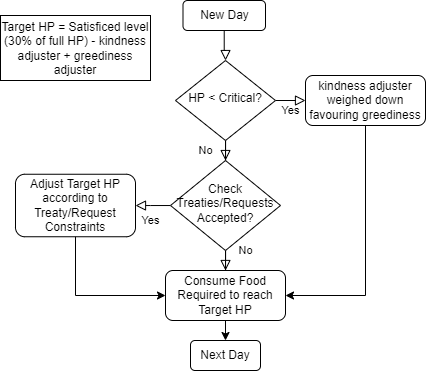
\includegraphics[scale=0.75]{009_team_7_agent_design/Images/v2.drawio.png}
    \end{center}
    \caption{Food taking decision flow chart.}
    \label{fig: operation flow chart}
\end{figure}

Upon completion of the memory bank updates and risk assessment routines, the agent then enters its food consumption routine. This routine runs only once per day when the platform is on the agent's floor. The routine begins by assessing whether the agent's health has been critical for multiple days, if this is the case the agent overrides any requests in effect and prioritises getting its health out of critical (Note however no treaties that prevent the agent from leaving critical HP would be accepted by the agent and thus no treaties would be broken at this point, treaty conditions are detailed in \Cref{subsec: Treaties}). The kindness adjuster is weighted down and the TakeFood function is executed. If the agent's health is not critical the routine evaluates whether it can abide within the constraints imposed for accepted treaties and requests. Once the constraints are in place the TakeFood function is executed in accordance to the greed and kindness adjusters within the bounds of the request/treaty constraints. 

Once the routine is complete the seenPlatform variable is reset to indicate the end of the day.

\subsection{Messages}
\label{subsec: Messages}
Although not a crucial feature of the final agent strategy - reasonable consideration went into deciding how to leverage messaging to better serve an agent during a simulation of the tower.

In order to think about how messaging could benefit the agent, two scenario's can be considered - one where the agent is sending messages to make an alert, enquiry or request and the converse, where an agent receives messages and can perform some action based on the incoming information or request.
\subsubsection{Sending Messages}
\label{subsubsec: Sending Messages}
The agent's behaviour is majorly determined by the intrinsic characteristics that constitute the agent's personality and so it was deemed that sending messages to gather information served no significant additional purpose as the new information would not have any influence on the next decision made. It is, however, important to benefit the collective effort of maintaining survival as a population - therefore an agent will send a reply to acknowledge information from other agent's and respond to requests stating whether they can comply.

\subsubsection{Receiving Messages}
\label{subsubsec: Receiving Messages}
The agent may adapt its behaviour upon receipt of request messages from other agent's. The criteria that must be met in order to comply with a request is as follows: 

\begin{itemize}
  \item The agent's extraversion rating must be higher than 5.
  \item The agent's kindness rating must be higher than it's greediness rating.
  \item The agent must not have been at critical health for \(\ge\) (the max \# of days at critical - 3).
\end{itemize}

If all of this criteria is met the agent will comply with the request, and it will reject the request if any of the conditions above are not met.

In all cases a truthful reply is sent from the agent to the message sender in an attempt to benefit the collective.

\subsection{Treaties}
\label{subsec: Treaties}
Treaties are the mechanism by which agents can communicate their needs to each other and organise themselves in way that is mutually beneficial.  

\subsubsection{Rejecting Proposed Treaties}
\label{subsec: Rejecting Treaties}
Treaties are rejected on the basis of certain criteria, these `conditions' reflect proposed treaties that are detrimental to the health of Team 7's agents at the expense of other agents. The following are the main criteria for rejecting treaties:

\begin{enumerate}
    \item 
    \textbf{Personality and behaviour traits:} \newline
    Treaties that are proposed to agents that have a less than average responsiveness are automatically rejected as this aligns with our aim to replicate human responses with agents. Note that responsiveness is an average of agreeableness, openness and extroversion. Thus most personality traits are taken into account. Similarly, an agent with conscientiousness less than 33\%\ lacks the intuition to plan for future events and thus is casual in its approach to treaties, resulting in viable treaties being rejected. This shows our commitment to having agents mirror their personality traits in the actions that they take.
    
    \item 
    \textbf{Unfavourable Condition Operators for Condition Types HP \&\ Available Food:} \newline
    If the condition type of a particular treaty is \textbf{HP} OR \textbf{Available Food} AND the the condition operator is \textbf{LE} OR \textbf{LT}, then the treaty is unfeasible for survival as an individual and/or collective. It is also unreasonable to assume realistic agents that mimic human behaviour would accept any alliances in which they were bound to a limited amount or percentage of food when their health is at the critical level. Thus all treaties that have the ability to put our agents in this position are rejected.
    
    \item 
    \textbf{Unfavourable Condition Operators for Condition Type Floor:} \newline
    If the condition type is \textbf{Floor} AND the the condition operator is \textbf{GE} OR \textbf{GT}, then the treaty is rejected. This is again due to the overwhelming risk agents are exposed to when they are on a floor with a scarcity of food and resources - they will likely be critical and thus shouldn't be bound by treaties that limit their food intake.
    
    \item 
    \textbf{Detrimental Request Operators:}\newline
    Any treaty, that uses the \textbf{LE} OR \textbf{LT} request operators will be rejected. This is due to the fact that the request types are concerned with leaving a certain amount or percentage of food and thus if being asked to limit the lower bound of our food intake, our agent may consume a larger than necessary amount/percentage of food and result in other agents starving to death. This ultimately defeats the purpose of self-organisation.
    
    \item 
    \textbf{Treaties active at the Critical Level:} \newline
    If the condition type holding up a certain treaty is \textbf{HP} and the condition value is less than the value required for the agent to be at the weak level, then such a treaty is not accepted. This is purely because of the risk it poses to our agent when we are below the weak level and require food but are bounded by a signed treaty that doesn't allow us to take any.
    
    \item 
    \textbf{Unreasonably long Duration of Treaties:} \newline
    The duration of the treaty is also an important consideration to take into account. For a treaty to be fully effective, it must persist for an adequate amount of time such that it is used beneficially for self-organisation. Therefore treaties in which our agents' actions are restricted for a long duration are rejected to avoid the negative impact these outdated treaties could have. 
    
    \item 
    \textbf{Clash of treaties:} \newline
    Each new treaty is compared to the existing active treaties that are already stored in the agent's memory. If a treaty is incompatible with those that are already active, then the agent will reject such treaties. For example: treaties that are based on the same request type cannot ask for conflicting amounts of food, for e.g. If a treaty asking us to leave exactly 10 units of food has been accepted, then a freshly proposed treaty requesting to leave less than 7 units of food has to be rejected to avoid conflict.
\end{enumerate}

Once a treaty is rejected, a confirmation of the rejection is sent to the proposer of the treaty and a message noting the outcome of the treaty is added to the log file at the output.

\subsubsection{Accepting Treaties}
\label{subsec: Accepting Treaties}

Treaties are accepted if the aforementioned rejection criteria are not satisfied and the agent has the relevant personality traits and behaviour. In particular, the responsiveness behaviour characteristic of a given agent should be greater than 50 and the personality trait conscientiousness should be greater than 33. 
\newline

All accepted treaties are stored in the active treaties field of the Base Agent thus allowing for the conflict criteria to be checked by iterating through the \texttt{activetreaties} map. Theoretically all treaties that get through the vetting process are either beneficial to the agent or the wider group and do not make the agent prone to an earlier than expected death as a result of accepting said treaty.

\subsubsection{Treaty Usage}
\label{subsec: Treaty Usage}
All treaties accepted are stored in the active treaties field of the base agent. Since treaties that could negatively impact the agent are rejected, ones that are signed can be followed, without further checking. 

Before an agent takes its share of food, The condition statements pertaining to active treaties are extensively checked to make sure that a treaty is being considered only when its respective conditions are upheld. Subsequently, the agent must check the request type, value, and operator. If the request type is \textit{LeavePercentFood}, it is converted to an \textit{amount} for easy comparison. 
The amount of food being taken is checked for compatibility with the amount of food that is to be left. If this is not the case then the \textit{foodtotake} variable for the agent is updated accordingly.
This will repeatedly happen until the expiration date of the treaty.

\subsubsection{Treaty Formulation}
\label{subsec: Treaty Formulation}
Treaty Formulation can play an important role in creating favourable conditions, not only for the survival of the proposing agent, but also for other agents. There are three types of scenarios which trigger the agent to propose a new treaty to its surrounding agents:

\begin{enumerate}
    \item \textbf{Health:} When an agent is in critical health state it is compelled to ask the neighbour above to leave an amount of food that can allow him to survive, i.e. go from critical to weak state. This health condition for this treaty is set such that the agents who sign the treaty are not put in danger, and this also makes it more likely for the treaty to be accepted.
    
    \item \textbf{Floor:} If the conscientiousness of the agent is a above a certain threshold, meaning that the agent is relatively forward thinking and aware of their surroundings, then the agent will try to initiate a treaty with the neighbouring agent above him. This is triggered upon a floor change when the current floor is at a lower level than the previous floor. A conscientiousness agent will know that it is likely that food will be more scarce at this level and so he initiates a treaty to make survival at this floor easier.

    \item \textbf{Propagation:} A treaty that has been accepted from an agent will be propagated onward in the same direction. If the treaty is coming from downwards and the request type is `LeaveAmountFood', then the request value is increased before propagating the same treaty upwards. This must be done to ensure that the agent above leaves enough food for our agent \textit{and} the agents below us. If the agent above uses the same strategy, then this can form an efficient means of survival for all agents in the tower.
\end{enumerate}

\section{Simulations and Analysis}
\subsubsection{Significance of Treaties}
\label{sec: Simulations and Analysis}
\Cref{fig: Cumulative Deaths without Treaties} and \Cref{fig: Cumulative Deaths with Treaties} illustrate the results from simulations with treaties disabled and enabled respectively. All other factors are left as default.

\begin{figure}[h!]
    \begin{center}
        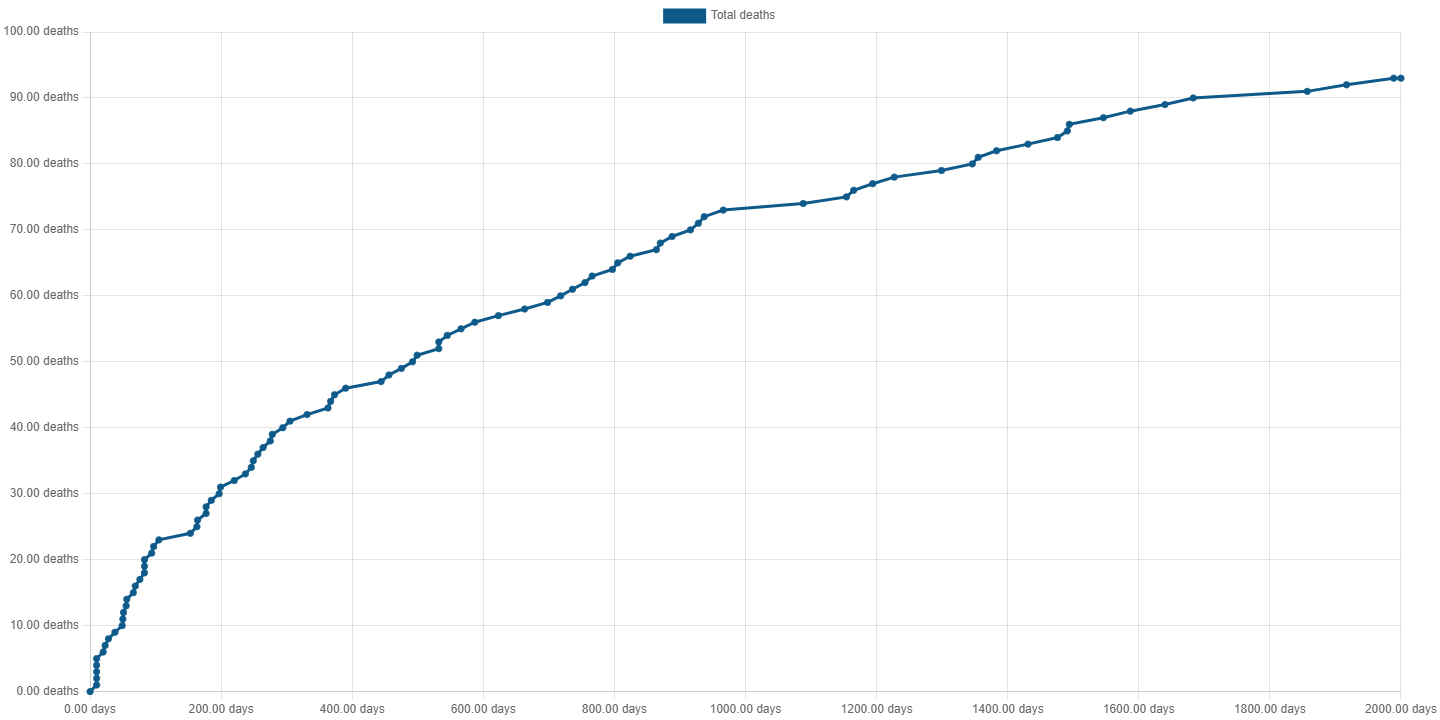
\includegraphics[scale=0.25]{009_team_7_agent_design/Images/Cumulative Deaths, WO Treaties, T7Only, 2000days, 20food, 93deaths.png}
    \end{center}
    \caption{Cumulative deaths without treaties (93 deaths).}
    \label{fig: Cumulative Deaths without Treaties}
\end{figure}

\begin{figure}[h!]
    \begin{center}
        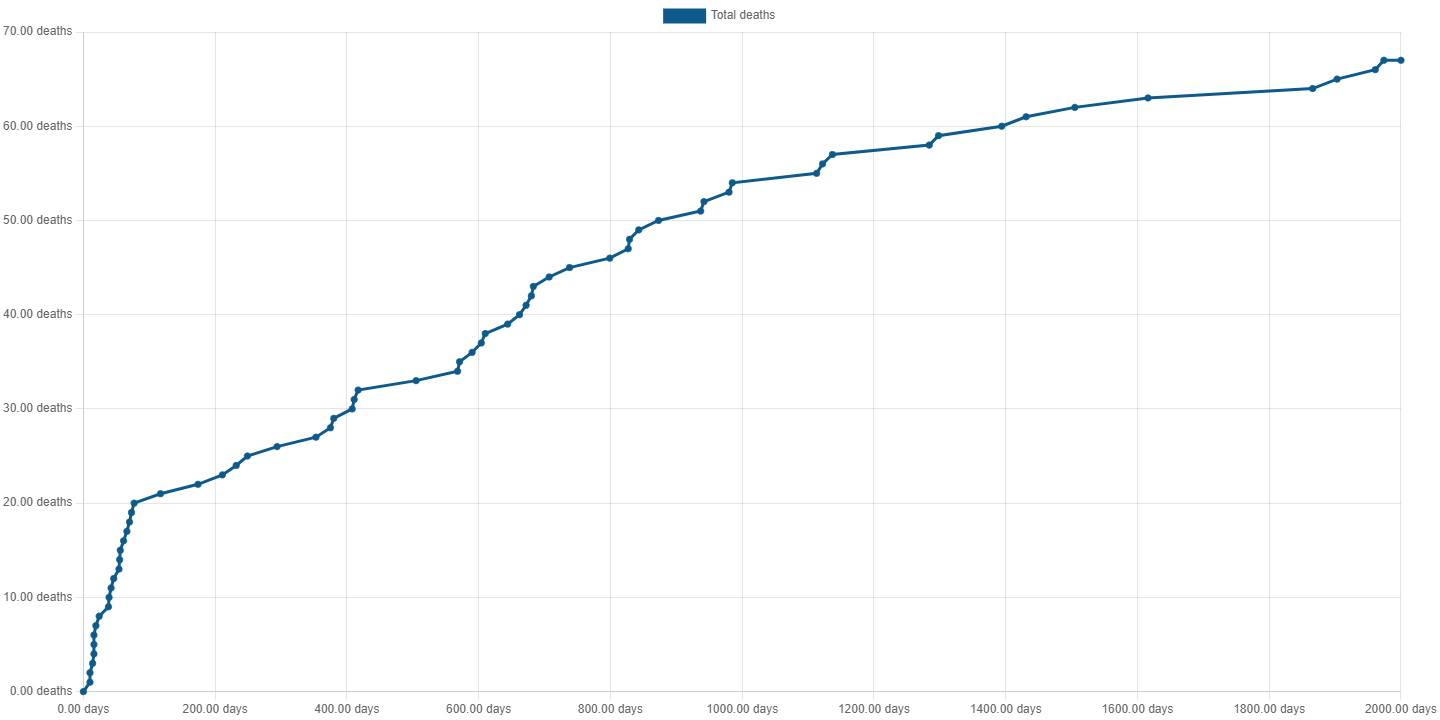
\includegraphics[scale=0.25]{009_team_7_agent_design/Images/Cumulative Deaths, With Treaties, T7Only, 2000days, 20food, 67deaths.png}
    \end{center}
    \caption{Cumulative deaths with treaties (67 deaths).}
    \label{fig: Cumulative Deaths with Treaties}
\end{figure}

This demonstrates that the agents perform better collectively when treaties are activated. This is expected as treaties enable agents to cooperate and organize the distribution of scarce food. 

\newpage
\subsubsection{Impact of Personalities}
\label{subsubsec: Impact of Personalities}

\subsubsection{Openness}
\label{subsubsec: Openness}

\Cref{fig: High Openness} and \Cref{fig: Low Openness} detail how our agents adapt to situations/scenarios differently based on varying levels of openness. In \Cref{fig: High Openness}, all the agents are spawned with openness values greater than 70 and in \Cref{fig: Low Openness}, the agents are spawned with openness values less than 30. All other personality traits are distributed as in the default case.

\begin{figure}[H]
    \begin{center}
        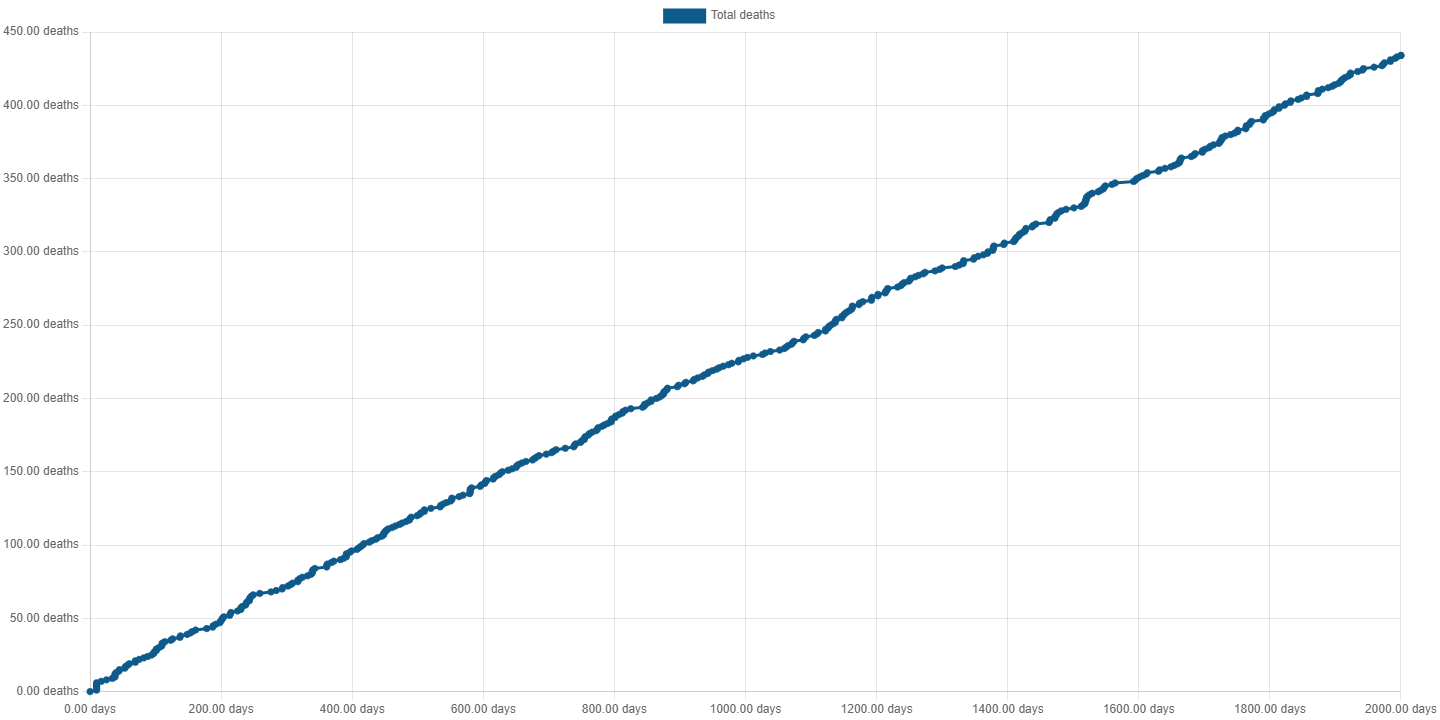
\includegraphics[scale=0.25]{009_team_7_agent_design/Images/Cumulative Deaths, With Treaties, T7Only, 2000days, 20food, High Openness, 434deaths.png}
    \end{center}
    \caption{Cumulative deaths with high openness (434 deaths).}
    \label{fig: High Openness}
\end{figure}

\begin{figure}[H]
    \begin{center}
        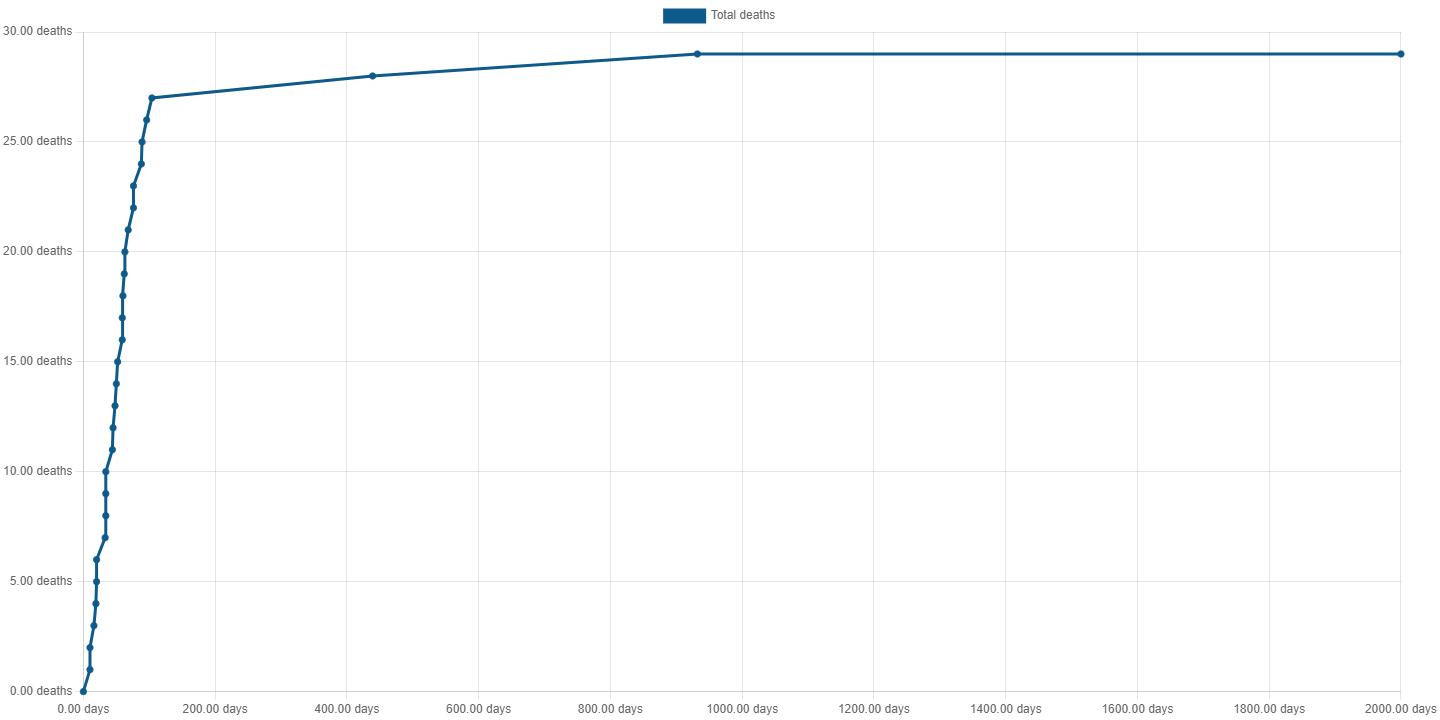
\includegraphics[scale=0.25]{009_team_7_agent_design/Images/Cumulative Deaths, With Treaties, T7Only, 2000days, 20food, Low Openness, 29deaths.png}
    \end{center}
    \caption{Cumulative deaths with low openness (29 deaths).}
    \label{fig: Low Openness}
\end{figure}

It can be observed that the agents collectively perform significantly better when openness is low, as a stabilising of the cumulative deaths curve can be seen for the agent with low openness. This can be explained by the fact that an agent with high openness will have a lower standard for accepting message requests and treaties - meaning they are more likely to agree to a request that is detrimental to their survival. Furthermore, an agent with a low openness value will be less welcoming to a change in floor and will therefore behave more cautiously. This will also improve the agents chances of survival. 

\subsubsection{Neuroticism}
\label{subsubsec: Neuroticism}

\Cref{fig: High Neuroticism} and \Cref{fig: Low Neuroticism} illustrate the results from simulations with agents with high neuroticism ($>$70) and low neuroticism ($<$30) respectively. All other traits are left as default.

\begin{figure}[H]
    \begin{center}
        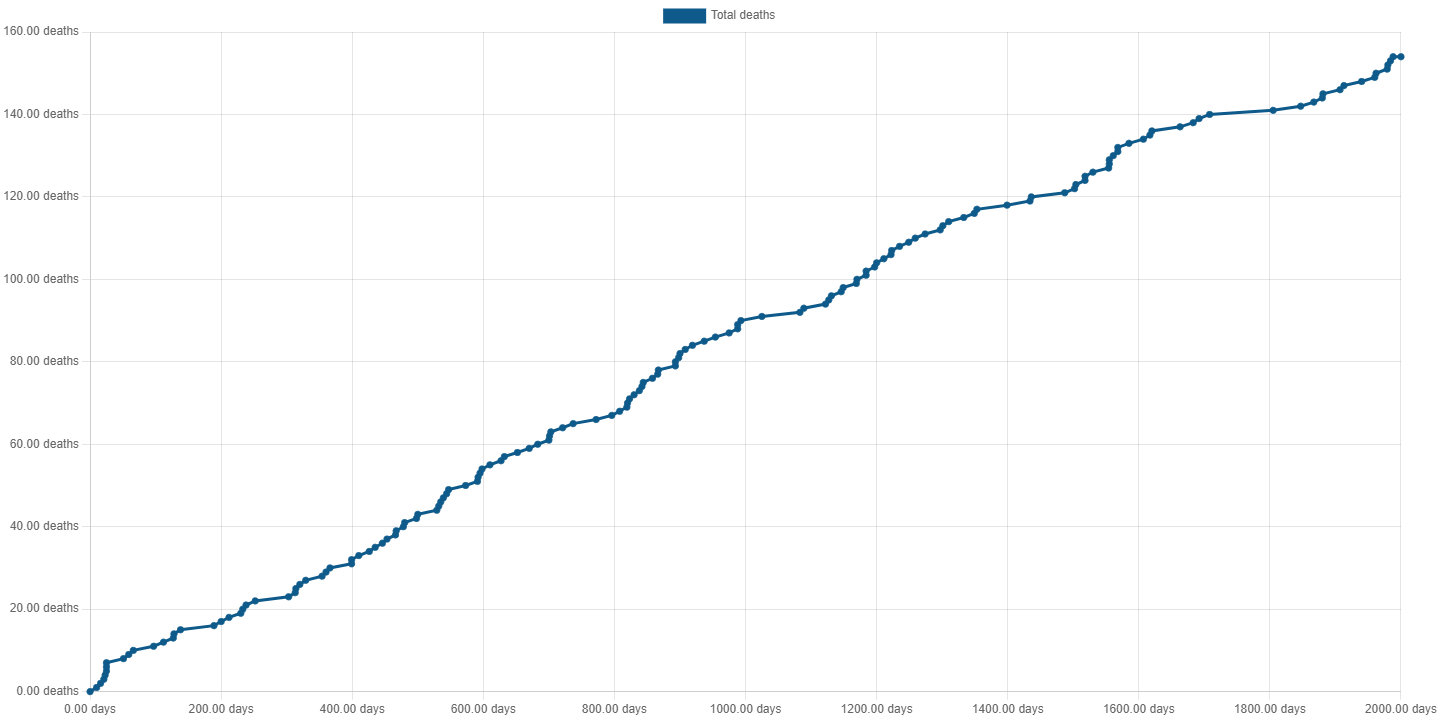
\includegraphics[scale=0.25]{009_team_7_agent_design/Images/Cumulative Deaths, With Treaties, T7Only, 2000days, 20food, High Neur, 154deaths.png}
    \end{center}
    \caption{Cumulative deaths with high neuroticism (154 deaths).}
    \label{fig: High Neuroticism}
\end{figure}

\begin{figure}[H]
    \begin{center}
        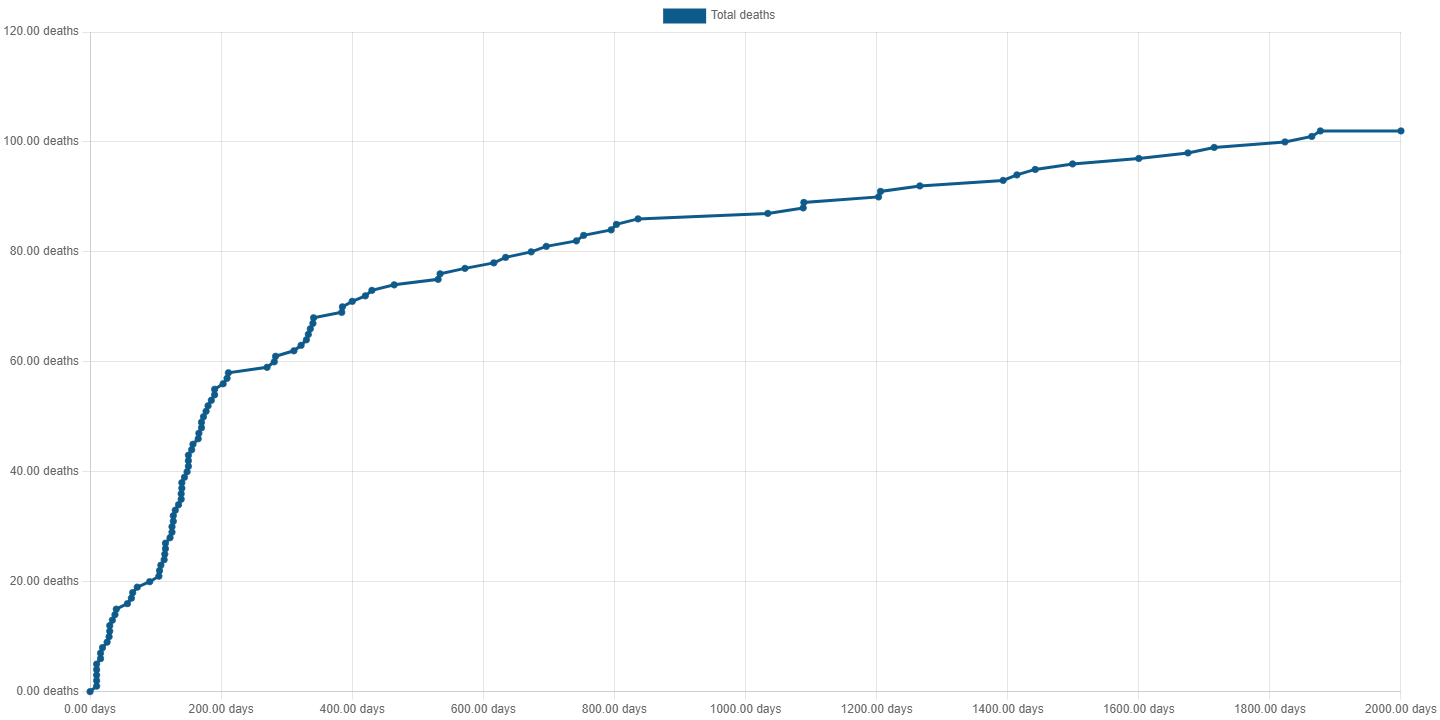
\includegraphics[scale=0.25]{009_team_7_agent_design/Images/Cumulative Deaths, With Treaties, T7Only, 2000days, 20food, Low Neur, 102deaths.png}
    \end{center}
    \caption{Cumulative deaths with low neuroticism (102 deaths).}
    \label{fig: Low Neuroticism}
\end{figure}

It can be seen that higher levels of neuroticism result in a greater number of agent deaths. This is expected as neuroticism results in volatility in an agents behaviour. 

\newpage
\subsubsection{Conscientiousness}
\label{subsubsec: Conscientiousness}

\Cref{fig: High Conscientiousness} and \Cref{fig: Low Conscientiousness} illustrate the results from simulations with agents with high conscientiousness ($>$70) and low conscientiousness ($<$30) respectively. All other traits are left as default.

\begin{figure}[H]
    \begin{center}
        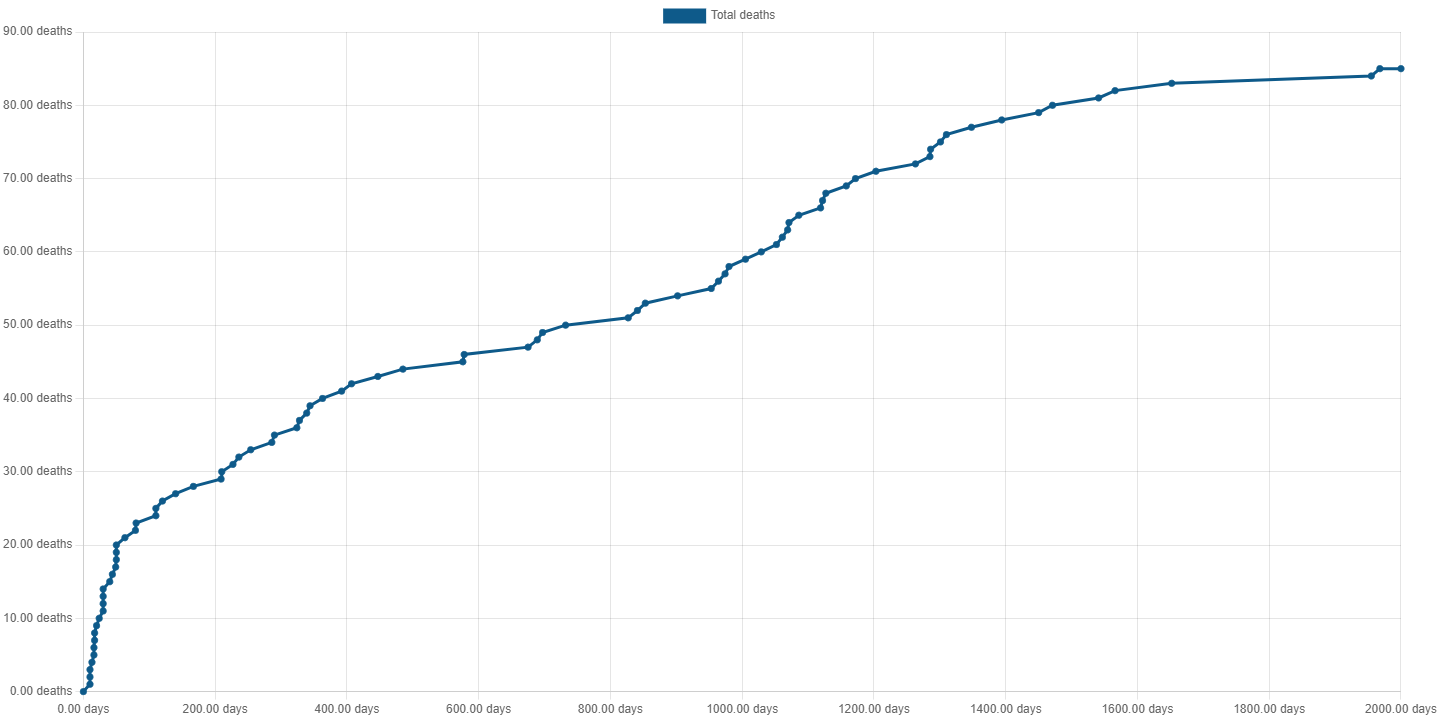
\includegraphics[scale=0.25]{009_team_7_agent_design/Images/Cumulative Deaths, With Treaties, T7Only, 2000days, 20food, High Conscient, 85deaths.png}
    \end{center}
    \caption{Cumulative deaths with high conscientiousness (85 deaths).}
    \label{fig: High Conscientiousness}
\end{figure}

\begin{figure}[H]
    \begin{center}
        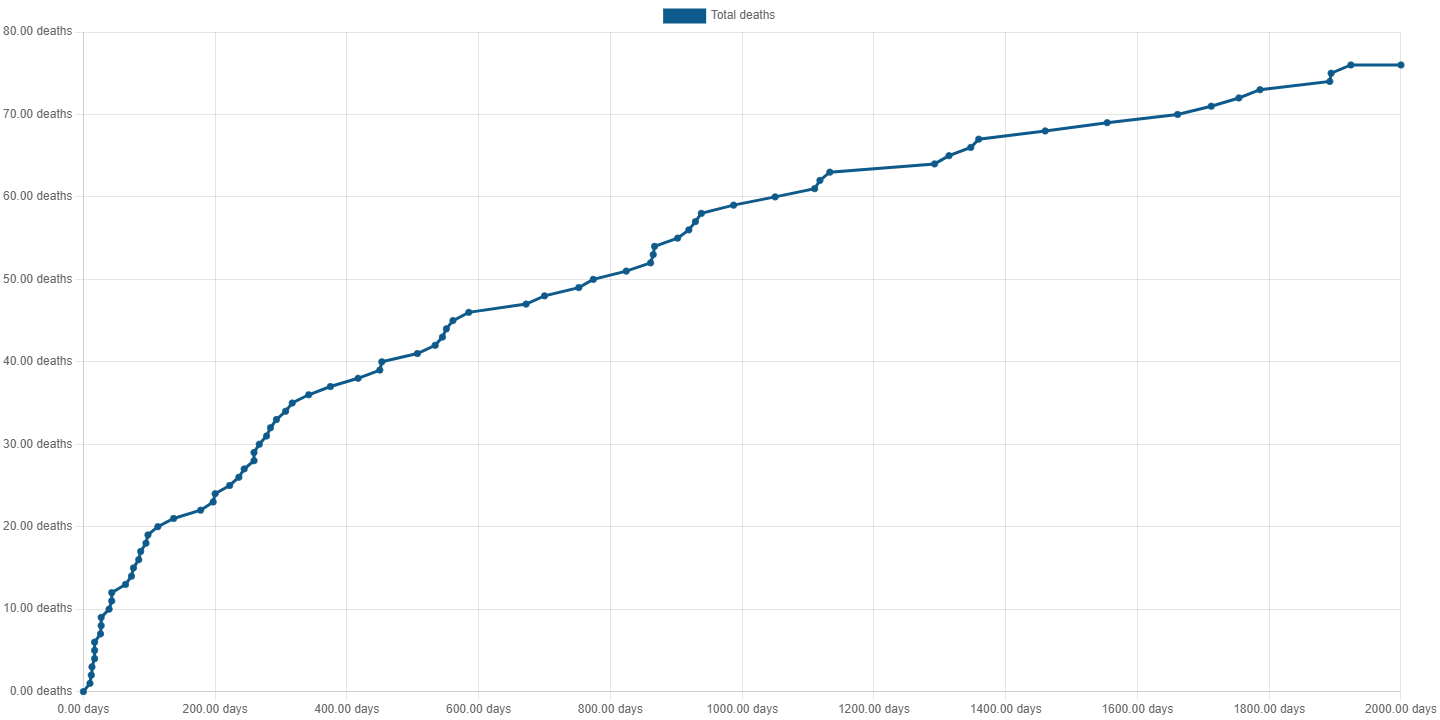
\includegraphics[scale=0.25]{009_team_7_agent_design/Images/Cumulative Deaths, With Treaties, T7Only, 2000days, 20food, Low Conscient, 76deaths.png}
    \end{center}
    \caption{Cumulative deaths with low conscientiousness (76 deaths).}
    \label{fig: Low Conscientiousness}
\end{figure}

It can be observed that there is no substantial difference in the number of deaths when the conscientiousness levels of the agents are collectively varied. This may indicate that the agent struggles to be strategic and that simply being more greedy can be a more effective route to survival. Ultimately, it would appear that other factors outweigh the impact of this personality trait. This is not entirely unreasonable as other personality traits may be more relevant to the given scenario. However, the expectation would be for deaths to reduce with higher conscientiousness although this is not generally observed. 

\newpage
\subsubsection{Extraversion}
\label{subsubsec: Extraversion}
\Cref{fig: High Extraversion} and \Cref{fig: Low Extraversion} illustrate the results from simulations with agents with high extraversion ($>$70) and low extraversion ($<$30) respectively. All other traits are left as default.

\begin{figure}[H]
    \begin{center}
        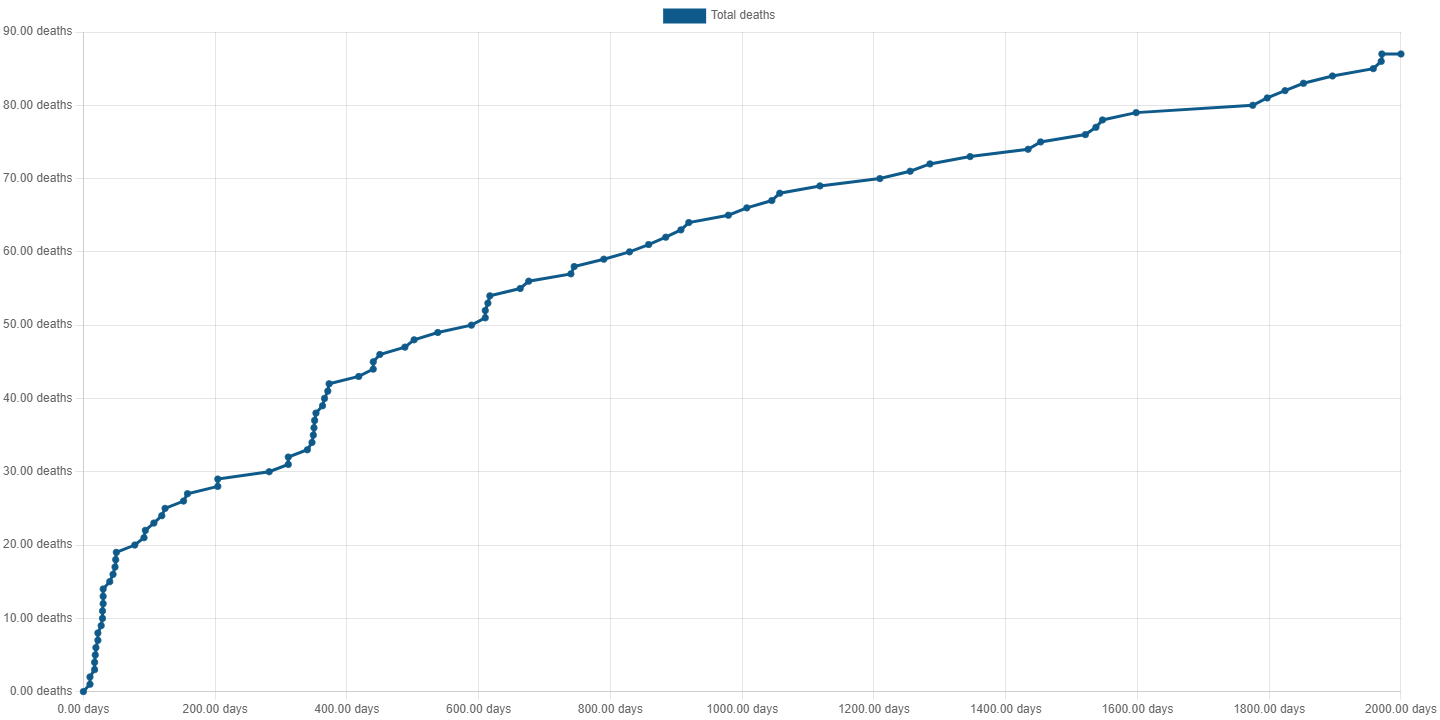
\includegraphics[scale=0.25]{009_team_7_agent_design/Images/Cumulative Deaths, With Treaties, T7Only, 2000days, 20food, High extra, 87deaths.png}
    \end{center}
    \caption{Cumulative deaths with high extraversion (87 deaths).}
    \label{fig: High Extraversion}
\end{figure}

\begin{figure}[H]
    \begin{center}
        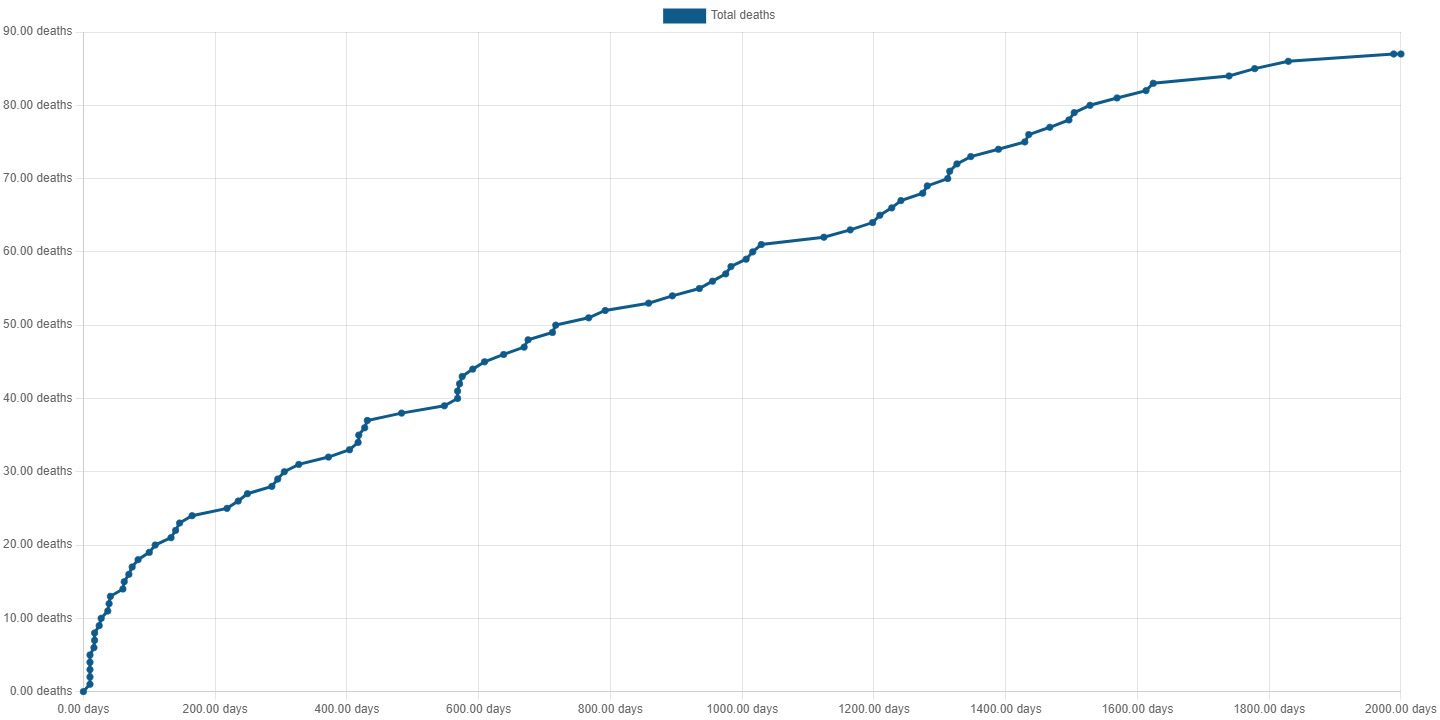
\includegraphics[scale=0.25]{009_team_7_agent_design/Images/Cumulative Deaths, With Treaties, T7Only, 2000days, 20food, Low extra, 87deaths.png}
    \end{center}
    \caption{Cumulative deaths with low extraversion (87 deaths).}
    \label{fig: Low Extraversion}
\end{figure}

Similar to extraversion, simulations show little variation in the number of deaths when the agents' extraversion values are collectively set to either high or low. This may suggest that other factors outweigh the impact of this personality trait. This is not unreasonable as other personality traits may be more relevant to the given scenario. In addition, it is difficult to predict what impact the extraversion level would have on the number of deaths. On one hand, higher extraversion levels will enable a greater number of treaties being signed. On the other hand, it may also result in treaties and requests of lower standards being accepted. These counteractive phenomenon may be the primary cause for the lack of variation in deaths.

\newpage
The following figures explore scenarios where the agents greediness and kindness are fixed before the food taking routine. 

\subsubsection{Greediness}
\label{subsubsec: Greediness}

\Cref{fig: Fixed High Greediness} and \Cref{fig: Fixed Low Greediness} illustrate the results from simulations with agents with high greediness ($>$70) and low greediness ($<$30) respectively. All other traits are left as default.

\begin{figure}[H]
    \begin{center}
        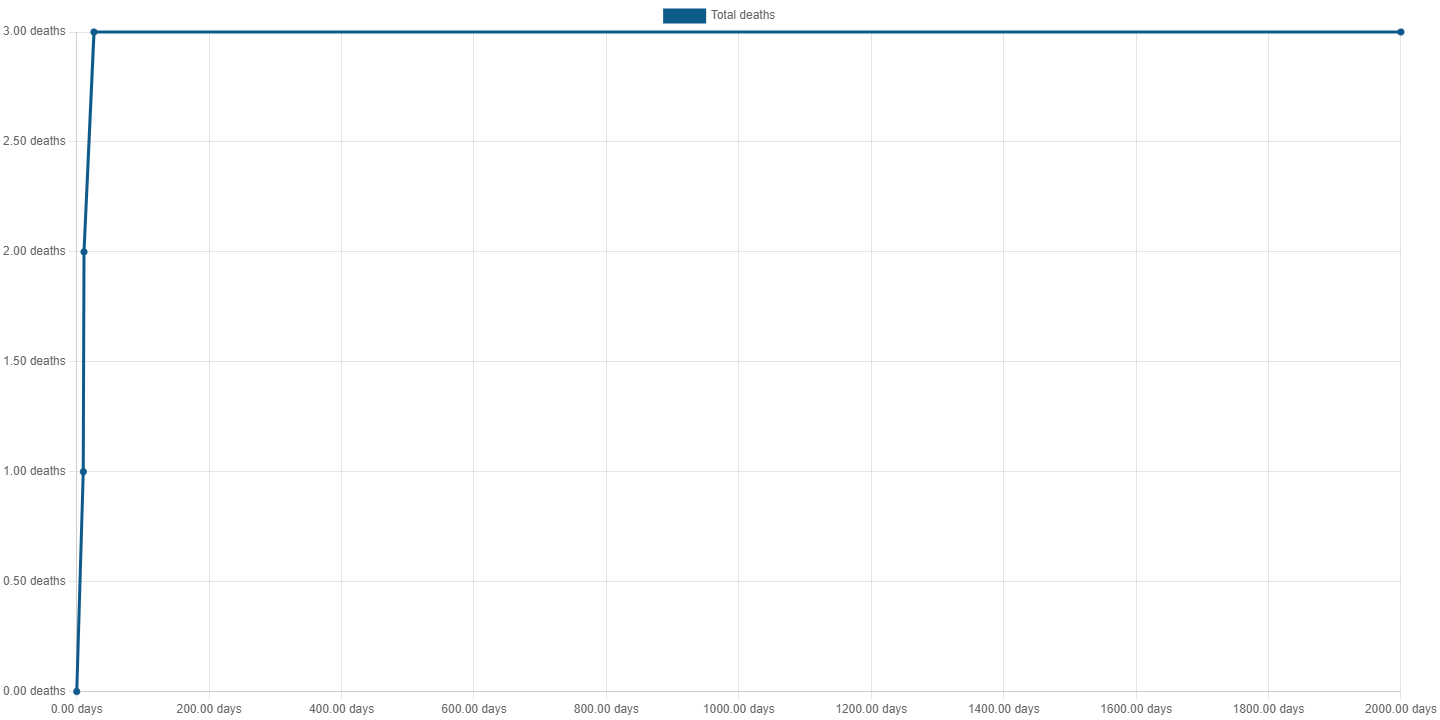
\includegraphics[scale=0.25]{009_team_7_agent_design/Images/Cumulative Deaths, fixed high greediness, T7Only, 2000days, 20food, 3deaths.png}
    \end{center}
    \caption{Cumulative deaths with high greediness (3 deaths).}
    \label{fig: Fixed High Greediness}
\end{figure}

\begin{figure}[H]
    \begin{center}
        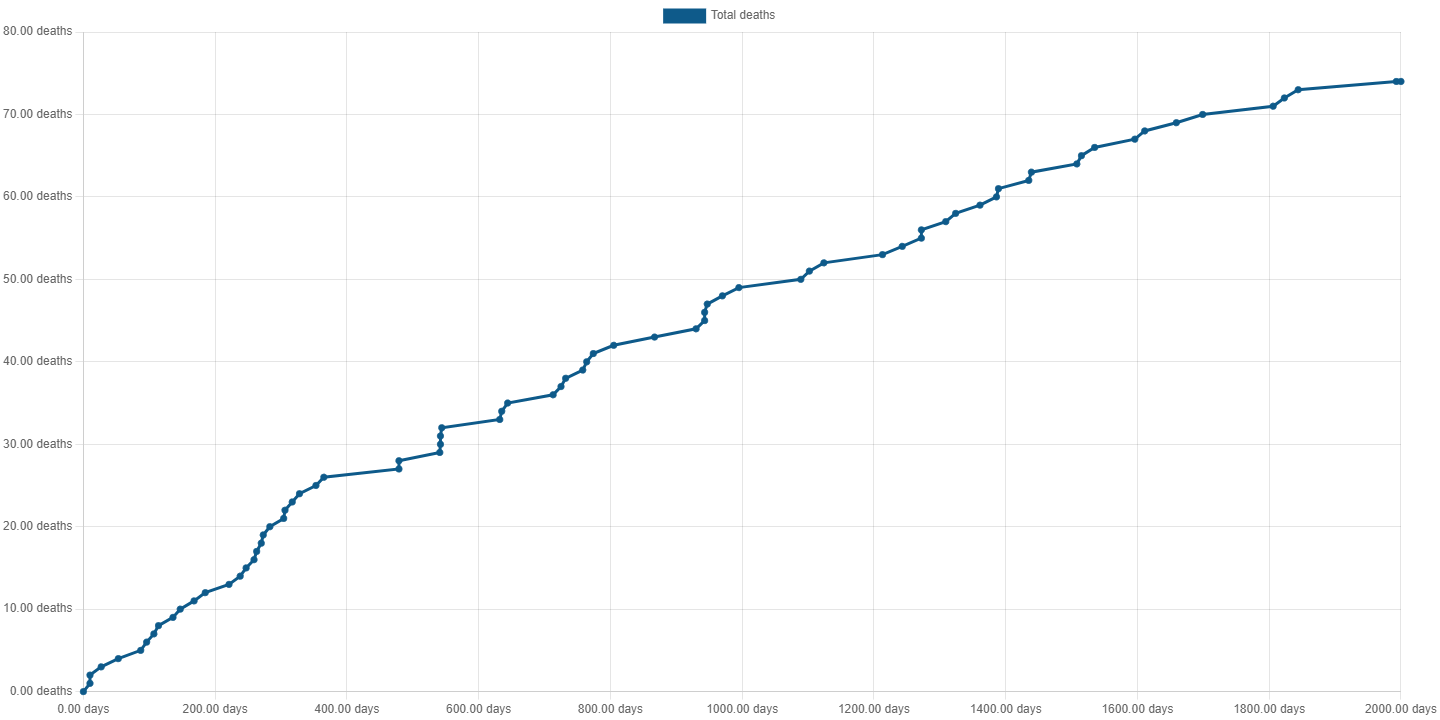
\includegraphics[scale=0.25]{009_team_7_agent_design/Images/Cumulative Deaths, fixed low greediness, T7Only, 2000days, 20food, 74deaths.png}
    \end{center}
    \caption{Cumulative deaths with low greediness (74 deaths).}
    \label{fig: Fixed Low Greediness}
\end{figure}

A tower housing agents with high greediness and enforceable (unbreakable) treaties capabilities show an extremely low death rate suggesting that such a group of agents are able to organise themselves quickly and stabilise the system. A low greediness score sees a dramatic increase in overall deaths and does not achieve stability over the 2000 day simulation.

\subsubsection{Kindness}
\label{subsubsec: Kindness}
\Cref{fig: Fixed High Kindness} and \Cref{fig: Fixed Low Kindness} illustrate the results from simulations with agents with high kindness ($>$70) and low kindness ($<$30) respectively. All other traits are left as default.

\begin{figure}[H]
    \begin{center}
        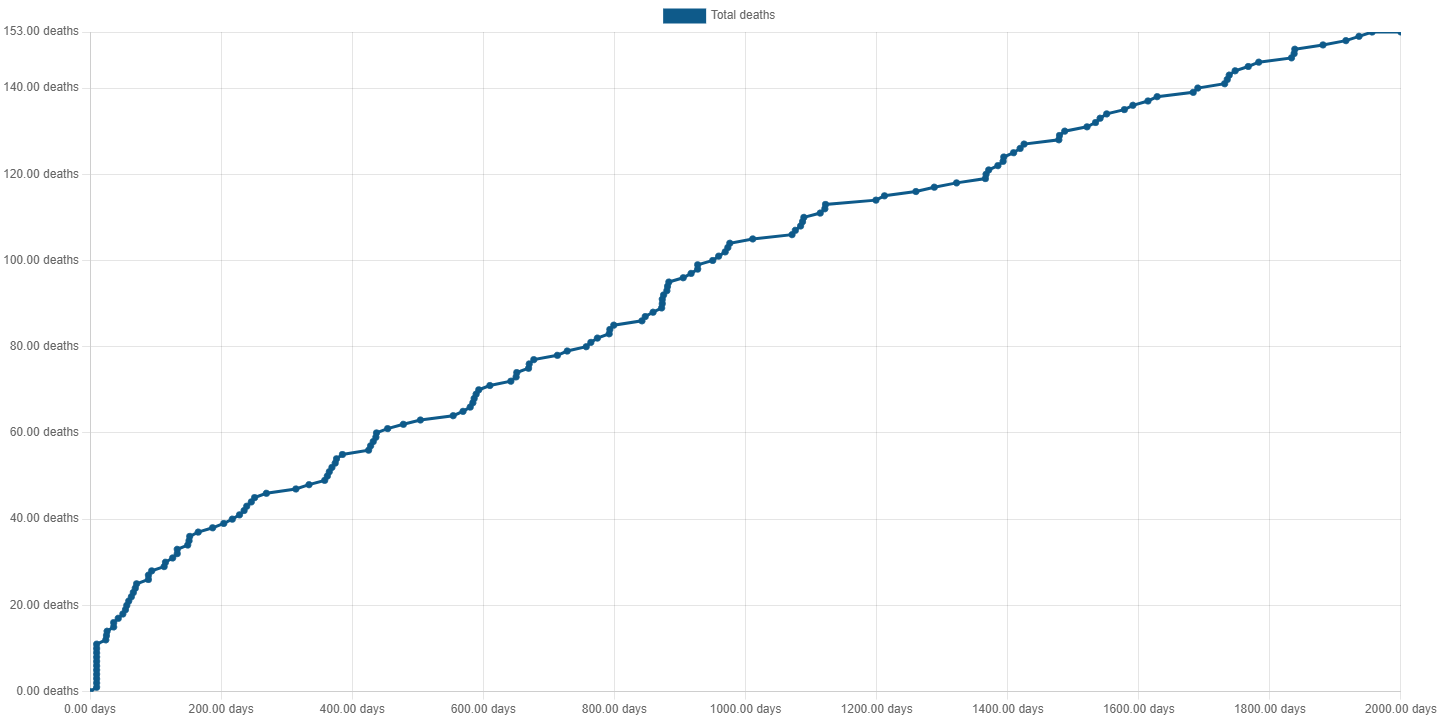
\includegraphics[scale=0.25]{009_team_7_agent_design/Images/Cumulative Deaths, fixed high kindness, T7Only, 2000days, 20food, 153deaths.png}
    \end{center}
    \caption{Cumulative deaths with fixed high kindness (153 deaths).}
    \label{fig: Fixed High Kindness}
\end{figure}

\begin{figure}[H]
    \begin{center}
        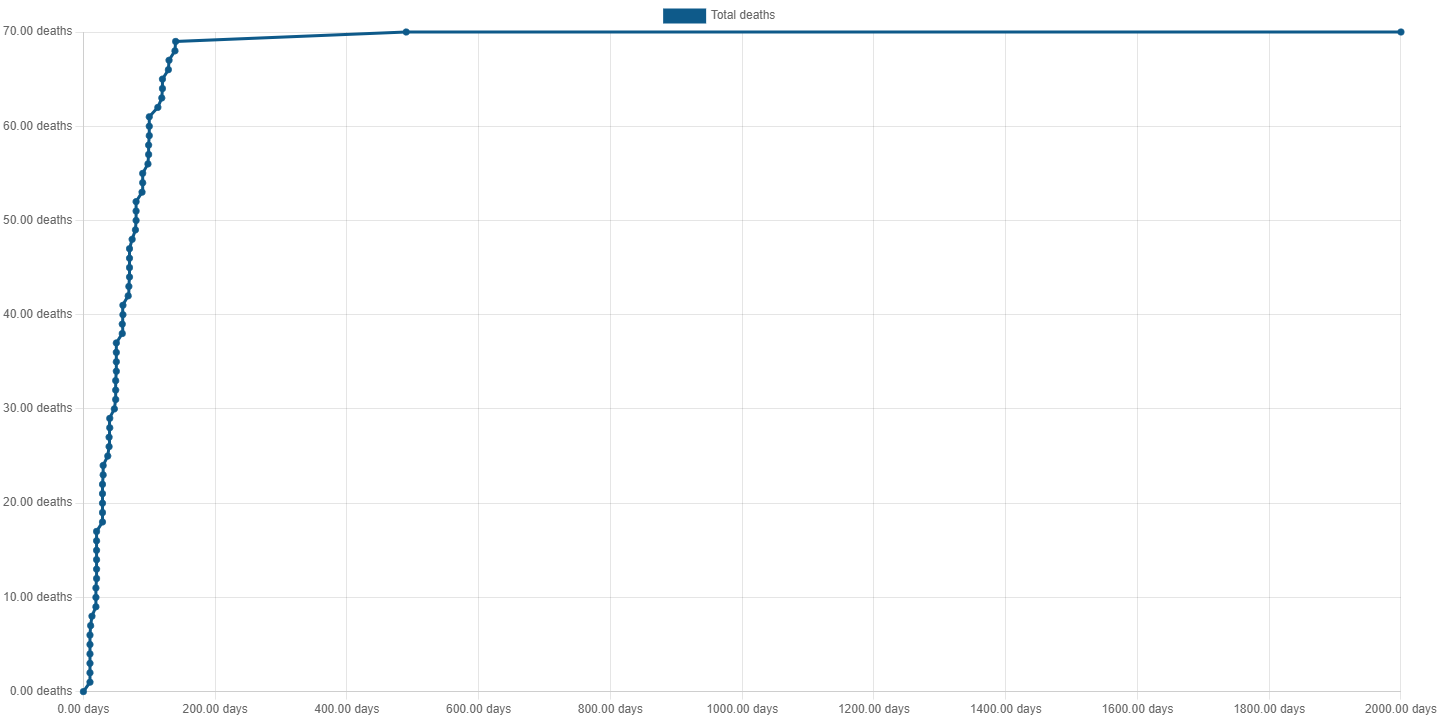
\includegraphics[scale=0.25]{009_team_7_agent_design/Images/Cumulative Deaths, fixed low kindness, T7Only, 2000days, 20food, 70deaths.png}
    \end{center}
    \caption{Cumulative deaths with fixed low kindness (70 deaths).}
    \label{fig: Fixed Low Kindness}
\end{figure}

A high kindness score sees double the deaths of a low kindness score. A high kindness score does not achieve stability however a low kindness score allows for the tower to reach in less than 200. The most likely explanation for this is that agents with a high kindness are potentially too selfless. It is likely that they consume in small quantities when food is available and thus do not have sufficient health when food isn't available. Thus, making them more vulnerable.

\subsubsection{Inter-team Comparison}
\Cref{tab: Inter-team data} shows the total number of deaths for simulations of various combinations of agent teams. All simulations are run with a simulation period of 500 days, shuffle period of 7 days and 10 team 7 agents with 10 agents of one other team type. The table is further broken down into food available per agent (5, 10 and 15).

\begin{table}
    \begin{center}
    \begin{tabular} { | m{4em} | m{6em} | m{4em} | m{4em} | m{4em} | }
        \hline
        \textbf{Agent Team} & \textbf{Food/Agent} & \textbf{Total Deaths} & \textbf{Team 7 Deaths} & \textbf{Other Deaths} \\
        \hline
        2 & 5 & 463 & 273 & 190 \\
        \hline
        2 & 10 & 149 & 80 & 49 \\
        \hline
        2 & 15 & 0 & 0 & 0 \\
        \hline
        3 & 5 & 347 & 183 & 164\\
        \hline
        3 & 10 & 73 & 53 & 20\\
        \hline
        3 & 15 & 0 & 0 & 0 \\
        \hline
        4 & 5 & 217 & 92 & 125\\
        \hline
        4 & 10 & 0 & 0 & 0 \\
        \hline
        4 & 15 & 0 & 0 & 0 \\
        \hline
        5 & 5 & 213 & 107 & 106 \\
        \hline
        5 & 10 & 5 & 5 & 0 \\
        \hline
        5 & 15 &  0 & 0 & 0 \\ 
        \hline
        6 & 5 & 459 & 136 & 323 \\
        \hline
        6 & 10 & 273 & 48 & 225 \\
        \hline
        6 & 15 & 126 & 24 & 102 \\
        \hline
    \end{tabular}
    \end{center}
    \caption{Comparison between agent teams and team 7.}
    \label{tab: Inter-team data}
\end{table}

\begin{figure}[H]
    \begin{center}
        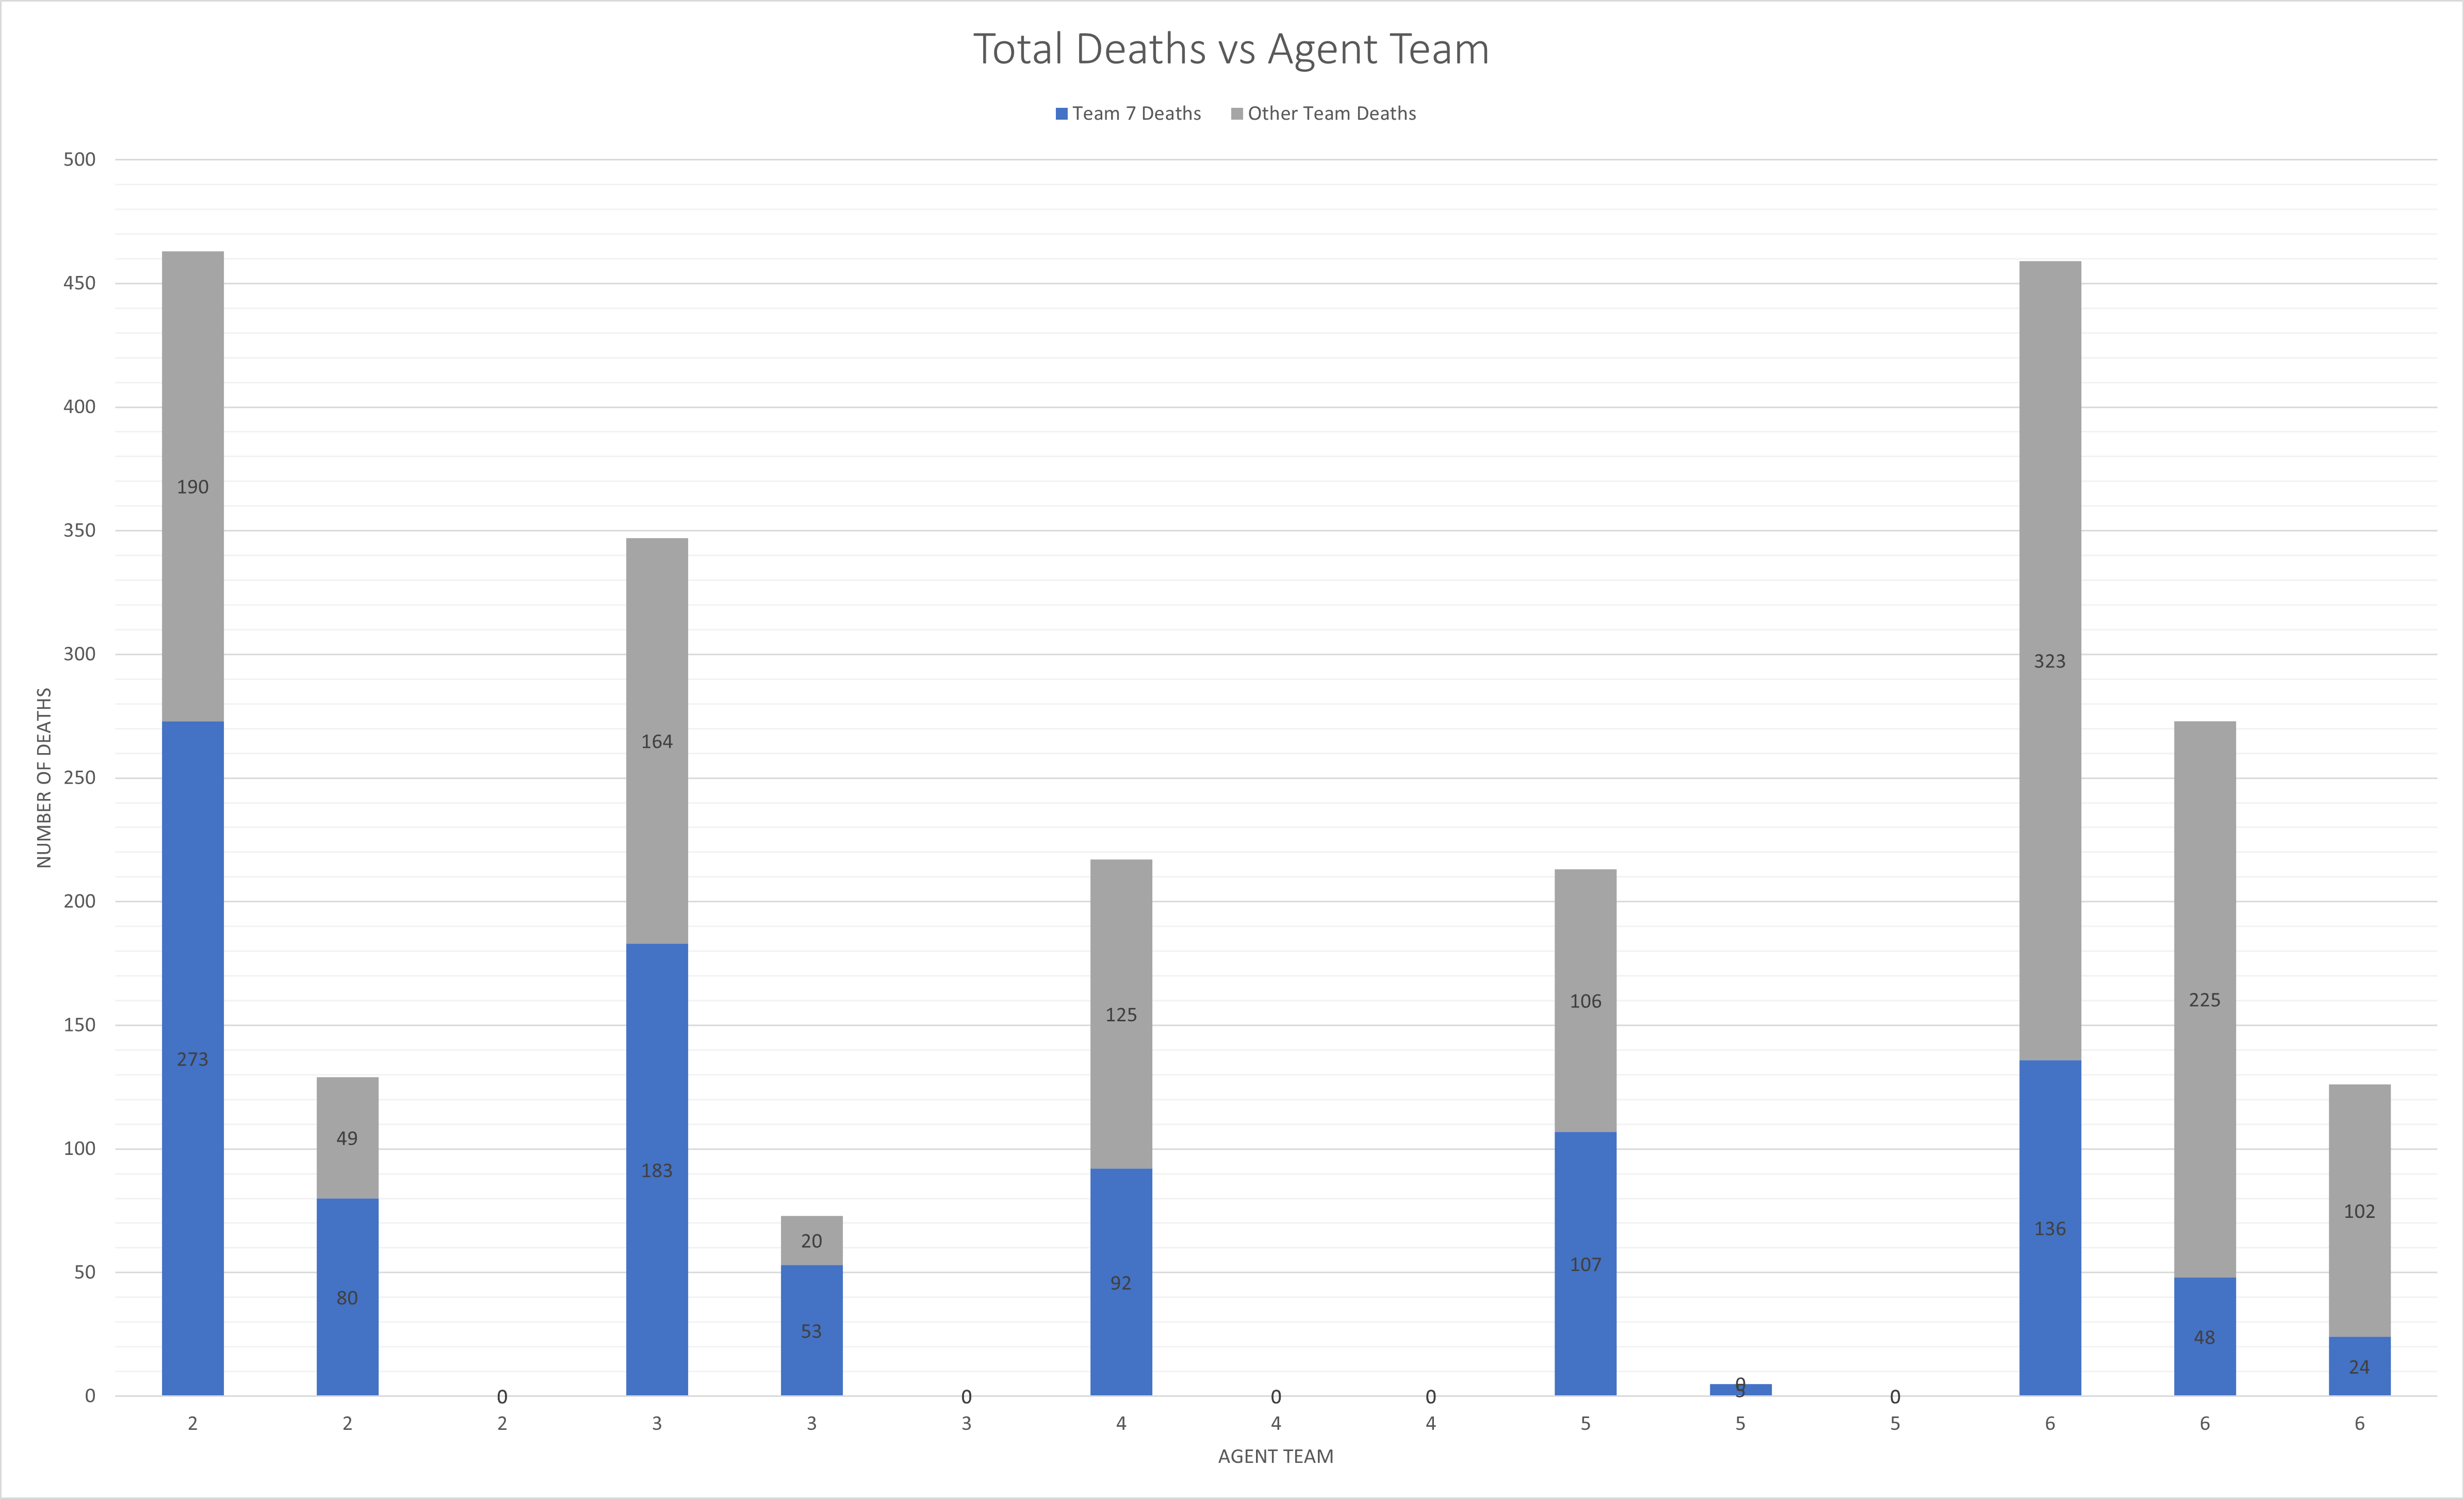
\includegraphics[scale=0.4]{009_team_7_agent_design/Images/Chart.png}
    \end{center}
    \caption{Deaths vs Agent Teams.}
    \label{fig: agent deaths}
\end{figure}

All team agents, bar team 6, were able to coexist with team 7 and achieve zero deaths for a food availability of 15 per agent, indicating that Team 6 agent was the most incompatible with our agent. Team 4 achieved zero deaths for food availability of 10 demonstrating a greater compatibility with team 7 and team 5's results are not too dissimilar.  

\subsubsection{Conclusion}
The agent designed by team 7 is unique in terms of the use of personalities to determine the general behaviour of the agent. These personality traits assigned allow it to mimic human behaviour as much as possible. The results presented above show that the team 7 can have a vastly different behaviours with each other agent, showing our compatibility with some agents and incompatibility with others. In short, the team 7 agent has been intricately designed to meaningfully engage in a huge variety of scenarios and attempt to accomplish its to major goals, to survive individually and collectively.